% !TeX program = xelatex
% !TeX encoding = UTF-8
% English translation in the complete IEICE Letter template.
% Working title; author details are reused from ../main.tex.
% Compile from this directory, or run build.ps1 from any directory.
\RequirePackage{iftex}
\RequireXeTeX
\makeatletter
\def\input@path{{../ieice_template/}}
\makeatother
\documentclass[letter]{ieice}

\usepackage{graphicx,xcolor}
\usepackage[fleqn]{amsmath}
\usepackage{tikz}
\usetikzlibrary{arrows.meta}
\usepackage{newtxtext}
\usepackage[varg]{newtxmath}

\usepackage[noadjust]{cite}
\renewcommand{\citepunct}{],\,\allowbreak[}
\renewcommand{\citedash}{]--\allowbreak[}
\makeatletter
\let\hyper@nopatch@caption\@empty
\makeatother
\usepackage[hidelinks,hyperfootnotes=false]{hyperref}

\setcounter{page}{1}
\field{A}
\title{Formal and Empirical Analysis of SAGA's Authorization Mechanism}
\authorlist{%
 \authorentry[1020268262@qq.com]{Anchen GAN}{n}{scnu}\MembershipNumber{}
 \authorentry{Libin WANG}{n}{scnu}\MembershipNumber{}
}
\affiliate[scnu]{The authors are with the School of Computer Science,
South China Normal University, Guangzhou 510631, China.}
% Manuscript dates and publication metadata are supplied by the journal.

\begin{document}
\maketitle
\begin{summary}
SAGA is a security architecture for AI agent systems. The formal analysis in the original SAGA study focused primarily on communication authentication and the confidentiality of Access Control Tokens (ACTs). We use Tamarin and TLA$^{+}$ to formally analyze SAGA's authorization mechanism and combine this analysis with experiments on the reference implementation. We identify three security issues: the contact-policy matching function fails to select the best-matching rule correctly, allowing a sender that should be denied to obtain an ACT; one-time public keys (OTKs) are not bound to the identities of the senders that retrieved them, allowing a sender permitted to communicate to establish new ACTs using OTKs retrieved and forwarded by other senders after exhausting its own OTK retrieval quota; and ACT validity checking and quota debit are not performed as a single atomic operation, allowing concurrent use of the same ACT to cause the receiving agent to process more requests than the ACT's initial request quota.
\end{summary}
\begin{keywords}
AI agents, SAGA, formal analysis, access control, protocol security
\end{keywords}

% !TeX root = main.tex
% !TeX program = xelatex
% Translation of the current Chinese introduction.

\section{Introduction}
\label{sec:introduction}

Multi-agent communication requires authentication of both parties and control over communication initiation and subsequent requests. SAGA (Security Architecture for Governing Agentic Systems)~\cite{syros2025saga} is a security architecture for AI (artificial intelligence) agents. Its contact policies determine whether a sender may retrieve a receiver's OTK (one-time public key) to obtain an ACT (access control token). Subsequent requests are constrained by the ACT's identity binding, validity period, and request quota.

The original SAGA study used ProVerif~\cite{blanchet2016proverif} to analyze agent--Provider authentication, inter-agent authentication, and ACT confidentiality~\cite{syros2025saga}. These properties do not guarantee correct authorization enforcement. Rule selection, OTK issuance and use, and concurrent ACT quota updates require separate analysis.

Using SAGA's protocol specification and reference implementation~\cite{syros2025sagaV2,sagaReferenceImpl2026}, we construct separate Tamarin~\cite{meier2013tamarin} models for contact-policy matching and OTK issuance and use. The policy model captures rule selection and subsequent authorization to check rule priorities and consistency with expected decisions. An independent evaluator and policy-evaluation results from the reference implementation cross-check its outputs. The OTK model checks whether keys are used by the senders to which they were issued and whether issuance limits constrain successful use of distinct OTKs. A TLA$^{+}$ (Temporal Logic of Actions) model~\cite{lamport2002specifying} checks ACT request quotas under concurrency. Reference-implementation experiments assess the effects of incorrect policy matching and ACT quota violations. We identify three issues:

(1) The matcher fails to select the most specific matching rule, allowing a sender that should be denied access to obtain an ACT.

(2) OTKs are not bound to the senders to which they are issued. An authorized sender can therefore obtain new ACTs using OTKs issued to and forwarded by other senders after exhausting its own retrieval quota.

(3) ACT validation and quota deduction do not form a single atomic operation. Concurrent connections can therefore cause the receiver to process more requests than the token's initial quota permits.

% !TeX root = main.tex
% !TeX program = xelatex
% Translation of the current Chinese workflow and analysis objectives.

\section{Authorization Workflow and Analysis Objectives}
\label{sec:authorization-workflow-objectives}

\subsection{Authorization Workflow}
\label{subsec:authorization-workflow}

Fig.~\ref{fig:saga-authorization-workflow} illustrates SAGA's authorization workflow. Let $P$ denote the Provider, $A$ the receiver, and $B$ the sender. Both agents are registered, with their identities bound to their credentials.

\begin{figure}[tb]
  \centering
  % !TeX root = saga_authorization_compact.tex
% Normal successful path, at native publication size: 80 mm x 95 mm.
% Symbols: k is A's OTK public key, t the encrypted ACT, K a local shared key.
% Source: SAGA v2 IV-D2/IV-E and saga/{agent.py,provider/provider.py}.
% K is never transmitted. No atomicity or original-retriever binding is implied.
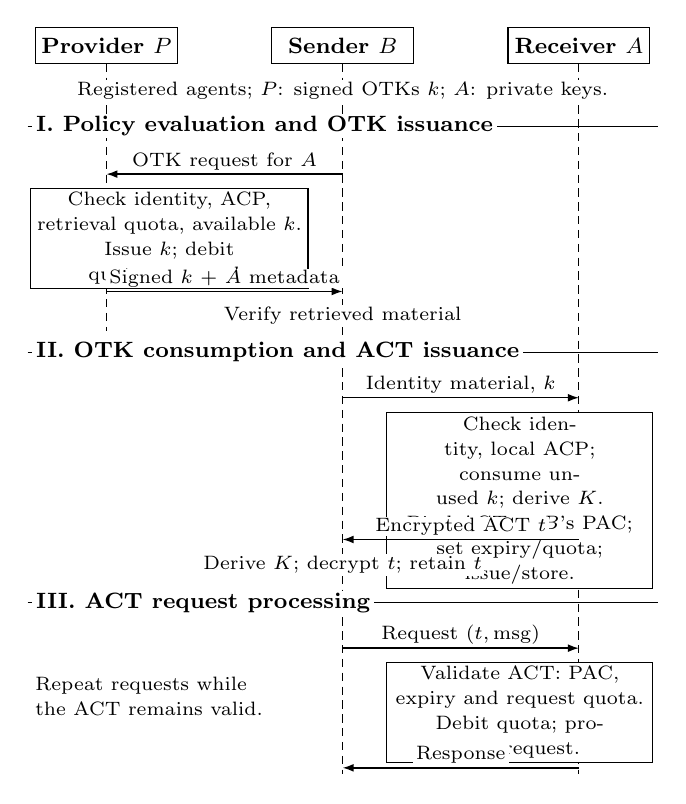
\begin{tikzpicture}[
  x=1mm,y=-1mm,
  font=\fontsize{7.5}{9}\selectfont,
  actor/.style={draw=black,line width=0.4pt,fill=white,
    minimum width=18mm,minimum height=4.6mm,inner sep=0pt,
    font=\bfseries\fontsize{8}{9.2}\selectfont},
  life/.style={draw=black,densely dashed,line width=0.4pt},
  msg/.style={-{Latex[length=1.4mm,width=1mm]},line width=0.5pt},
  wire/.style={fill=white,inner xsep=0.4mm,inner ysep=0.15mm},
  local/.style={draw=black,line width=0.4pt,fill=white,
    align=center,inner xsep=0.6mm,inner ysep=0.55mm,anchor=north},
  senderstep/.style={fill=white,align=center,inner sep=0.3mm},
  phase/.style={anchor=west,fill=white,inner xsep=0.5mm,
    inner ysep=0.2mm,font=\bfseries\fontsize{8}{9.2}\selectfont}
]
  \path[use as bounding box] (0,0) rectangle (80,95);
  \draw[life] (10,4.6) -- (10,38.5);
  \draw[life] (40,4.6) -- (40,94.8);
  \draw[life] (70,4.6) -- (70,94.8);
  \node[actor] at (10,2.3) {Provider $P$};
  \node[actor] at (40,2.3) {Sender $B$};
  \node[actor] at (70,2.3) {Receiver $A$};
  \node[fill=white,inner sep=0.2mm] at (40,8)
    {Registered agents; $P$: signed OTKs $k$; $A$: private keys.};

  \draw[line width=0.4pt] (0,12.5) -- (80,12.5);
  \node[phase] at (0.5,12.5) {I. Policy evaluation and OTK issuance};
  \draw[msg] (40,18.6) -- node[wire,above=0.3mm]
    {OTK request for $A$} (10,18.6);
  \node[local,text width=34mm] at (18,20.3) {
    Check identity, ACP,\\
    retrieval quota, available $k$.\\
    Issue $k$; debit quota; remove $k$.
  };
  \draw[msg] (10,33.5) -- node[wire,above=0.3mm]
    {Signed $k$ + $A$ metadata} (40,33.5);
  \node[senderstep] at (40,36.6) {Verify retrieved material};

  \draw[line width=0.4pt] (0,41.2) -- (80,41.2);
  \node[phase] at (0.5,41.2) {II. OTK consumption and ACT issuance};
  \draw[msg] (40,47) -- node[wire,above=0.3mm]
    {Identity material, $k$} (70,47);
  \node[local,text width=32.6mm] at (62.5,48.8) {
    Check identity, local ACP;\\
    consume unused $k$; derive $K$.\\
    Bind ACT to $B$'s PAC;\\
    set expiry/quota; issue/store.
  };
  \draw[msg] (70,65) -- node[wire,above=0.3mm]
    {Encrypted ACT $t$} (40,65);
  \node[senderstep] at (40,68.2) {Derive $K$; decrypt $t$; retain $t$};

  \draw[line width=0.4pt] (0,73) -- (80,73);
  \node[phase] at (0.5,73) {III. ACT request processing};
  \draw[msg] (40,78.8) -- node[wire,above=0.3mm]
    {Request $(t,\mathrm{msg})$} (70,78.8);
  \node[local,text width=32.6mm] at (62.5,80.5) {
    Validate ACT: PAC,\\
    expiry and request quota.\\
    Debit quota; process request.
  };
  \draw[msg] (70,94) -- node[wire,above=0.3mm]
    {Response} (40,94);
  \node[anchor=north west,align=left,fill=white,
    text width=32mm,inner sep=0.4mm] at (0.5,82) {
    Repeat requests while\\
    the ACT remains valid.
  };
\end{tikzpicture}

  \caption{Authorization workflow of SAGA.}
  \label{fig:saga-authorization-workflow}
\end{figure}

The receiver's ACP (Agent Contact Policy) defines contact permission through AID (agent identifier) patterns and budgets. When multiple rules match, the most specific matching rule determines the budget. Agent $A$ uploads pre-generated, signed OTK public keys to $P$ and retains the corresponding private keys. The Provider verifies the sender's registered identity and TLS (Transport Layer Security) client certificate, determines its OTK retrieval quota from the contact policy, and maintains the remaining quota for each sender~\cite{syros2025sagaV2,sagaReferenceImpl2026}.

After verifying the retrieved material, $B$ establishes a TLS connection with $A$ and uses the OTK to request an ACT. Agent $A$ consumes the unused OTK, derives a shared key from the corresponding private key and $B$'s PAC (public access control key), and issues an ACT bound to that PAC with a validity period and an initial request quota. Agent $B$ derives the same key using its private access control key and the OTK, decrypts the ACT, and retains the ciphertext and token metadata~\cite{syros2025sagaV2,sagaReferenceImpl2026}.

Subsequent requests carry the ACT ciphertext and are subject to identity binding, expiration, and remaining request quotas. An ACT can be reused across connections, with identity, local contact permission, and ACT validity checked at each new connection. The sender and receiver maintain separate local request quotas, and connections using the same ACT share the receiver's remaining quota. The ACT request quota is independent of the OTK retrieval quota maintained by $P$~\cite{sagaReferenceImpl2026}.

\subsection{Analysis Objectives}
\label{subsec:analysis-objectives-assumptions}

We examine three aspects of this authorization workflow.

\textbf{ACP:} Contact policies determine a sender's communication permission and OTK retrieval quota from its identity and policy rules. We examine whether matching respects rule priorities and authorization decisions conform to the specified policy~\cite{syros2025sagaV2,sagaReferenceImpl2026}.

\textbf{OTK:} The Provider issues an OTK, which the receiver consumes when issuing an ACT. We examine the identity and authorization conditions governing OTK issuance, use, and ACT issuance, including issuance limits and one-time consumption.

\textbf{ACT:} An ACT restricts subsequent requests through identity binding, a validity period, and a request quota. We examine token validation, request processing, and quota updates to assess quota enforcement.

% !TeX root = main.tex
% !TeX program = xelatex
% Definitions are tied to the archived inputs identified in the source comments.

\section{Formal Modeling and Verification Setup}
\label{sec:formal-modeling-analysis-setup}

Authorization in SAGA involves contact-policy matching, OTK issuance and use, and ACT request-quota control. For these three stages, we construct an independent policy evaluation program, a Tamarin symbolic model, and a TLA$^{+}$ quota model, respectively, and use ProVerif and TLC to examine the corresponding security properties.

\subsection{Contact-Policy Evaluation and Verification}
\label{subsec:policy-evaluation-model}

A contact policy determines the OTK retrieval quota from the sender's AID and an ordered rule set. To independently examine the matching function in the reference implementation, we implement a separate policy evaluation program that selects the best-matching rule according to SAGA's rule priorities. The program supports three rule types: the universal wildcard rule (\texttt{*}), exact lowercase ASCII AIDs, and name-wildcard rules with a fixed UID (\texttt{uid:*}). Their scores are $0$, $4|UID|+8|name|$, and $4|UID|+2$, respectively. Among matching rules, the program selects the rule with the highest score and returns its budget; if no rule matches, it returns a budget of $0$. It produces no evaluation result if a rule falls outside the supported syntax or if the highest score is tied.

The independent policy evaluation program treats a budget greater than $0$ as permission and a budget less than or equal to $0$ as denial. In the reference implementation, the Provider's \texttt{/access} interface rejects OTK issuance when the budget is less than or equal to $0$, whereas the receiver's local policy check rejects only when the budget is less than $0$~\cite{sagaReferenceImpl2026}.

The independent policy evaluation program supplies the expected results, while the actual return values of the matching function in the reference implementation supply the implementation-side results. Comparisons use the same sender AID and ordered rule set. The input contents, rule order, and implementation version are recorded to check agreement in rule selection and returned budgets.

To analyze how differences in policy decisions affect subsequent communication, we provide the ProVerif model with a scenario in which the independent policy evaluation program denies access but the matching function in the reference implementation permits it. The existing communication protocol model is used to check the correspondence between request-acceptance events and prior token-issuance events, as well as the reachability of request-acceptance events. The corresponding ProVerif queries are as follows:

\noindent\begin{minipage}{\linewidth}
\renewcommand{\verbatimsize}{\small}
\begin{verbatim}
query receiver: bitstring, sender: bitstring,
      tok: bitstring, msg: bitstring;
    event(ChatAccept(receiver, sender, tok, msg))
    ==> event(TokenIssue(receiver, sender, tok)).

query receiver: bitstring, sender: bitstring,
      tok: bitstring, msg: bitstring;
    event(ChatAccept(receiver, sender, tok, msg)).
\end{verbatim}
\end{minipage}

Experiments based on the reference implementation further examine how policy decisions affect the actual authorization process. They include three scenarios: both sides allow (A/A), both sides deny (D/D), and the independent policy evaluation program denies access while the reference implementation permits it (D/A). Execution records the policy-matching results at the Provider and receiver and the Provider's \texttt{/access} response. The experiments also check OTK issuance, OTK handling at the receiver, ACT issuance and storage, and the sender's decryption and metadata checks on the returned ACT.

\subsection{OTK Issuance and Use Model}
\label{subsec:otk-issuance-use-model}

The Provider maintains OTK retrieval quotas, while the receiver maintains OTK consumption state. The Tamarin model represents these two states separately and checks whether the sender that actually uses an OTK is the same sender that previously retrieved it from the Provider. The model includes Provider $P$, receiver $A$, and senders $B,C$. Initially, $A$ holds two OTKs, and $B$ and $C$ each have a nonrenewable quota for retrieving one OTK.

Linear facts represent the Provider's retrieval quotas, OTKs available for issuance, and OTKs not yet consumed by the receiver. Issuing an OTK consumes the corresponding retrieval credit and available key at the Provider, while issuing an ACT consumes the corresponding OTK at the receiver. Senders retain obtained OTK public keys through persistent facts. The correspondence between each participant's identity and its public access-control key (PAC) is established as an initial fact. Private messages containing the identities of both communicating parties represent communication protected by TLS. The cryptographic abstraction uses the DH equational theory, a hash KDF with a domain-separation tag, and ideal symmetric encryption. The ACT ciphertext contains the sender's PAC to retain the binding between the token and the identity.

The threat model allows $B$ to forward an OTK public key that it has retrieved to $C$. After exhausting its own OTK retrieval quota, $C$ can still use an OTK forwarded by $B$ to request an ACT with its own registered identity, PAC, and private key. Each OTK can be forwarded at most once. In the baseline configuration, both the Provider and receiver permit $B,C$. Control configurations disable OTK forwarding or have both sides deny $C$.

Tamarin uses protocol events to record the execution relationships among OTK issuance, ACT issuance, client decryption, and application-request acceptance. The model first checks the original bound on OTK issuance and the unique issuance and consumption of each OTK. It additionally checks whether the identity that retrieves an OTK matches its actual user's identity and whether a sender successfully uses at most one distinct OTK. The following Tamarin lemma expresses identity correspondence between the sender that retrieved an OTK and the sender that uses it:

\begingroup
\renewcommand{\verbatimsize}{\footnotesize}
\setlength{\verbatimbaselineskip}{10pt}
\noindent\begin{minipage}{\linewidth}
\begin{verbatim}
lemma successful_use_requires_issue_to_same_sender:
  "All a s k t pac #i.
     RequestAccepted(a, s, k, t, pac) @i
     ==> (Ex #j.
       ProviderIssue(a, s, k) @j & j < i)"
\end{verbatim}
\end{minipage}
\endgroup

Here, \texttt{ProviderIssue} denotes an OTK-issuance event at the Provider, and \texttt{RequestAccepted} denotes an event in which the receiver accepts an application request. The property requires each successfully accepted request to be traceable to an earlier issuance of the corresponding OTK to the same sender. Auxiliary lemmas also check OTK issuance and consumption counts and whether the corresponding ACT issuance and client decryption occur before a request is accepted.

\subsection{Concurrent ACT Request Quota Model}
\label{subsec:act-quota-model}

The ACT request-quota model uses TLA$^{+}$ to describe execution when multiple connections share the request quota of the same ACT. At initialization, the sender and receiver store the same ACT, and their quota states are both set to the token's initial quota. The receiver's shared balance represents the ACT's remaining request quota; each connection's state variables record its request-processing stage. The sender's balance and message-delivery state describe processing at both ends.

When a connection is established, the receiver checks the token metadata and remaining quota. After parsing a request, it checks the token metadata and positive balance again, moving the connection into the checked state. The model represents token-validity checking and quota debit as two separate atomic actions, corresponding to two independently locked critical sections in the reference implementation~\cite{sagaReferenceImpl2026}. The quota-debit action requires the connection to have passed the check and updates the shared balance after the lock is reacquired, without checking whether the current balance is still positive. The debit uses \texttt{Clamp} to keep the balance nonnegative and increments the connection's count of requests for which quota debit has completed. Because checking and debiting do not form one atomic operation, other connections can execute between the two actions. The TLA$^{+}$ action is defined as follows:

\begingroup
\renewcommand{\verbatimsize}{\footnotesize}
\setlength{\verbatimbaselineskip}{10pt}
\noindent\begin{minipage}{\linewidth}
\begin{verbatim}
Clamp(n) == IF n < 0 THEN 0 ELSE n

ADebit(c) ==
    /\ apc[c] = "Checked"
    /\ receiverRemaining' =
        Clamp(receiverRemaining - 1)
    /\ counts' = [counts EXCEPT ![c].admits = @ + 1]
    /\ apc' = [apc EXCEPT ![c] = "Debited"]
    /\ UNCHANGED
        <<senderRemaining, bpc, link, faultCount>>
\end{verbatim}
\end{minipage}
\endgroup

The model sums the number of requests for which quota debit has completed across all connections and checks whether the cumulative quota-debit count exceeds the ACT's initial request quota. The quota-safety invariant is defined in TLA$^{+}$ as follows:

\begingroup
\renewcommand{\verbatimsize}{\footnotesize}
\setlength{\verbatimbaselineskip}{10pt}
\noindent\begin{minipage}{\linewidth}
\begin{verbatim}
Accepted ==
    SumOn([c \in Connections |-> counts[c].admits],
          Connections)

ReceiverQuotaSafety == Accepted <= InitialQuota
\end{verbatim}
\end{minipage}
\endgroup

Here, \texttt{Accepted} denotes the total number of requests for which connections have completed quota debit. TLC checks this request-quota safety invariant, the model's state types, and consistency between balances and request counts. The finite-state check sets the initial request quota to $1$, uses two connections, permits each connection to submit at most one request, and keeps the token metadata valid.

% !TeX root = main.tex
% !TeX program = xelatex
% English translation of the current Chinese results chapter.

\section{Verification Results and Security Analysis}
\label{sec:results}

The analysis of SAGA's authorization process identifies three issues: the contact-policy matcher fails to select the best-matching rule, OTKs are not bound to the identities of the senders that retrieved them, and concurrent ACT requests can exceed their quotas. The following subsections present the verification results, concrete counterexamples, and causes of these issues.

\subsection{Incorrect Contact-Policy Matching}
\label{subsec:policy-evaluation-consistency}

The value returned by the contact-policy matching function depends on rule order, potentially allowing a sender that should be denied to obtain communication permission. For the identity \texttt{alice@example.com:agent}, the rule \texttt{alice@example.com:*} has a budget of $-1$, whereas the wildcard rule \texttt{*} has a budget of $10$. Under the best-matching-rule priority requirement, the specific rule should be selected and a budget of $-1$ returned regardless of the order of these two rules. However, when the specific rule precedes the wildcard rule, the matching function in the reference implementation returns $10$; reversing their order yields $-1$.

This error arises because the matching function fails to update the current best-matching rule correctly. When the function matches the specific rule, it updates the budget but does not update \texttt{best\_pattern}. Consequently, the subsequent wildcard rule's score of $0$ is still compared with the initial best score of $-1$, ultimately overwriting the budget with $10$~\cite{sagaReferenceImpl2026}.

In the scenario where the independent policy evaluation program returns denial and the actual matching function returns permission, ProVerif returns \texttt{false} for the \texttt{ChatAccept} event reachability query, indicating an execution path that triggers this event. The correspondence query between request acceptance and token issuance returns \texttt{true}, indicating that every request-acceptance event is preceded by a token-issuance event for the same receiving agent, sending agent, and token. Thus, an execution path exists in which an application request is accepted after token issuance.

Experiments based on the reference implementation further examine the effect of this error on the actual authorization process. In the scenario where the independent policy evaluation program denies access but the reference implementation allows it (D/A), the matching functions at both the Provider and the receiving agent return a budget of $10$. The Provider returns HTTP 200 for the \texttt{/access} request and issues an OTK, after which the receiving agent consumes the OTK and issues and stores an ACT. The sending agent successfully decrypts the returned ACT, whose contents match the record stored by the receiving agent. In the scenario where both sides deny access (D/D), the Provider returns a budget of $-1$ and rejects the request with HTTP 403. When both sides allow access (A/A), ACT issuance and storage complete normally.

The Provider and the receiving agent use the same matching function, causing both sides to fail to enforce the best-matching-rule priority requirement and ultimately allowing a sender that should be denied to obtain an ACT.

\subsection{OTKs Are Not Bound to Their Requesters}
\label{subsec:otk-issuance-use}

Tamarin finds that, after exhausting its own OTK retrieval quota, a sending agent can still establish a new ACT using an OTK retrieved by another identity. In the configuration that permits OTK transfer and in which both the Provider and the receiving agent allow $B,C$ to communicate, the Provider issues one OTK to $B$ and one to $C$.

$C$ first uses the OTK issued to it by the Provider to complete ACT issuance, decryption, and acceptance of the first application request. The Provider then refuses further issuance because $C$ has exhausted its retrieval quota. $B$ transfers its own retrieved but unconsumed OTK to $C$, which requests another ACT using its own registered identity, access-control public key, and private key, and successfully decrypts the token. The receiving agent subsequently accepts the first application request associated with this ACT. Thus, the Provider has issued $1$ OTK to $C$, whereas $C$ has successfully used $2$ distinct OTKs.

Tamarin returns \texttt{verified} for the existential query, confirming that this execution trace is reachable. For the remaining properties, Tamarin returns \texttt{verified} for the Provider's per-sender limit on OTK issuance, unique issuance and consumption of each OTK, and the correspondence between request acceptance and preceding ACT issuance and client decryption.

When checking consistency between the identity to which an OTK was issued and the identity that actually uses it, Tamarin returns \texttt{falsified}, indicating an execution trace in which communication is successfully established using an OTK retrieved by another sender. In the configuration with a retrieval quota of $1$, the property that a sender successfully uses at most one distinct OTK also returns \texttt{falsified}. These results show that the Provider's original per-sender limit on OTK issuance still holds, but this limit does not prevent a sender from obtaining new ACTs using OTKs retrieved by other identities.

When OTK transfer is disabled, the normal communication paths of $B,C$ remain reachable, and the two additional security properties return \texttt{verified}. When both the Provider and the receiving agent deny $C$, the communication and OTK-transfer paths for $C$ are unreachable, whereas normal communication by $B$ remains reachable; both properties again return \texttt{verified}.

The issue is that the Provider maintains OTK retrieval quotas by sender identity, but an issued OTK is not itself bound to the identity of the sender that retrieved it. When issuing an ACT, the receiving agent checks the current connection's identity, local contact permission, and whether the OTK has been consumed. However, because the OTK carries no binding information associated with the identity that retrieved it, these checks cannot determine whether the current sender retrieved that OTK. Consequently, even after exhausting its own OTK retrieval quota, $C$ can still use an OTK transferred by $B$ to request and obtain a new ACT under its own identity.

\subsection{ACT Request Quota Exceeded under Concurrency}
\label{subsec:act-concurrent-quota}

When multiple connections concurrently use the same ACT, the cumulative quota-debit count can exceed the token's initial quota. For a configuration with an initial quota of $1$, two connections, and one request submitted by each connection, TLC detects a violation of the \texttt{ReceiverQuotaSafety} invariant and generates a counterexample trace containing $13$ states.

In state $11$, connections $c_1$ and $c_2$ have both completed token checking, while the receiving agent's remaining quota is still $1$. Connection $c_1$ then executes \texttt{ADebit}, reducing the remaining quota to $0$ and increasing the cumulative quota-debit count to $1$. Connection $c_2$ subsequently executes the same action. The remaining quota stays at $0$, but the cumulative quota-debit count increases to $2$, exceeding the initial quota. TLC therefore reports a violation of the quota-safety invariant.

Concurrent experiments based on the reference implementation further observe backend-call counts exceeding the ACT's initial request quota. With an initial quota of $50$, submitting $51$ requests sequentially produces $50$ backend calls. For the concurrent execution, $49$ requests are first processed sequentially. A thread barrier then ensures that two connections both pass the check against the single remaining unit of quota before continuing with quota debit. The experiment records $51$ backend calls and a remaining quota of $0$, with the same result in three repetitions.

ACT validity checking and quota debit are not completed within the same atomic operation. The function \texttt{token\_is\_valid()} checks the token and remaining quota while holding a lock, then releases the lock. The function \texttt{receive\_conversation()} subsequently reacquires the lock and debits the quota, but does not check the current remaining quota again. Two connections can therefore pass validity checking before either debit occurs, then each complete a quota debit and proceed to subsequent request processing. Because \texttt{Clamp} keeps the debit result nonnegative, the balance cannot fall below zero, but the cumulative quota-debit count can still exceed the ACT's initial quota.

% !TeX root = main.tex
% !TeX program = xelatex
% English translation of the current Chinese discussion and conclusion.

\section{Discussion and Conclusion}
\label{sec:discussion-conclusion}

This study analyzes SAGA's authorization process and identifies three issues. First, the contact-policy matching function fails to update the current best-matching rule correctly while traversing the rules. Its result consequently depends on rule order, potentially allowing a sender that should be denied to obtain an ACT. Second, OTKs are not bound to the identities of the senders that retrieved them, allowing a sender that has exhausted its own OTK retrieval quota to establish new ACTs using OTKs retrieved by other senders. Finally, ACT validity checking and quota debit are not completed within the same atomic operation. Multiple concurrent requests can therefore pass checking against the same remaining quota, causing the cumulative quota-debit count to exceed the ACT's initial quota.

The ProVerif analysis demonstrates the effect of incorrect policy matching on subsequent request acceptance. Tamarin provides reachable traces in which OTKs retrieved by other senders are transferred and used, while the TLA$^{+}$ model and reference-implementation experiments confirm the concurrent execution that exceeds the ACT quota. These results indicate that SAGA's authorization security depends not only on communication authentication and ACT confidentiality, but also on correct contact-policy matching, binding OTKs to the identities of the senders that retrieved them, and performing ACT validity checking and quota debit within the same atomic operation.


\bibliographystyle{../ieice_template/ieicetr}
\bibliography{../references}
\end{document}
